\documentclass[12pt]{article}
\usepackage{fancyhdr}
\usepackage{amsmath,amsfonts,enumerate}
\usepackage{color,graphicx}
\usepackage{tikz}
\usepackage{pgfplots}
\usepackage{listings}
\usepackage{algorithm}
\usepackage{algorithmic}
\usetikzlibrary{arrows,positioning,shapes,calc,matrix}
\pagestyle{fancy}
%%%%%%%%%%%%%%%%%%%%%%%%%%%%%%%%%%%%%%%%%%%%%%%%%
% Course customization based on Professor's teaching
%%%%%%%%%%%%%%%%%%%%%%%%%%%%%%%%%%%%%%%%%%%%%%%%%
\newcommand{\masunitnumber}{CENG 403}
\newcommand{\examdate}{January 2025}
\newcommand{\academicyear}{2024-2025}
\newcommand{\semester}{I}
\newcommand{\coursename}{Deep Learning - CNN Architectures \& RNN Introduction}
\newcommand{\numberofhours}{3}
%%%%%%%%%%%%%%%%%%%%%%%%%%%%%%%%%%%%%%%%%%%%%%%%%
% CUSTOM SPACING COMMANDS FOR ANSWER SPACES
%%%%%%%%%%%%%%%%%%%%%%%%%%%%%%%%%%%%%%%%%%%%%%%%%
\newcommand{\answerspace}[1]{\vspace{#1}}
\newcommand{\questionspace}{\vspace{3cm}}        
\newcommand{\subquestionspace}{\vspace{2.5cm}}   
\newcommand{\shortanswer}{\vspace{2cm}}          
\newcommand{\mediumanswer}{\vspace{3cm}}         
\newcommand{\longanswer}{\vspace{4cm}}           
\newcommand{\journalspace}{\vspace{4.5cm}}       
\newcommand{\codespace}{\vspace{5cm}}            
%%%%%%%%%%%%%%%%%%%%%%%%%%%%%%%%%%%%%%%%%%%%%%%%%
% Header setup
%%%%%%%%%%%%%%%%%%%%%%%%%%%%%%%%%%%%%%%%%%%%%%%%%
\lhead{}
\rhead{}
\chead{{\bf MIDDLE EAST TECHNICAL UNIVERSITY}}
\lfoot{}
\rfoot{}
\cfoot{}
\begin{document}
\setlength{\headsep}{5truemm}
\setlength{\headheight}{14.5truemm}
\setlength{\voffset}{-0.45truein}
\renewcommand{\headrulewidth}{0.0pt}
\begin{center}
SEMESTER \semester\ EXAMINATION \academicyear
\end{center}
\begin{center}
{\bf \masunitnumber\ -- \coursename}
\end{center}
\vspace{20truemm}
\noindent \examdate\hspace{45truemm} TIME ALLOWED: \numberofhours\ HOURS
\vspace{19truemm}
\hrule
\vspace{19truemm}
\noindent\underline{INSTRUCTIONS TO CANDIDATES}
\vspace{8truemm}
%%%%%%%%%%%%%%%%%%%%%%%%%%%%%%%%%%%%%%%%%%%%%%%%%%%%%%
% Instructions based on professor's emphasis
%%%%%%%%%%%%%%%%%%%%%%%%%%%%%%%%%%%%%%%%%%%%%%%%%%%%%%
\begin{enumerate}
\item This examination paper contains {\bf SIX (6)} questions and comprises 
{\bf EIGHT (8)} printed pages.
\item Answer all questions. 
The marks for each question are indicated at the beginning of each question.
\item Answer each question beginning on a {\bf FRESH} page of the answer book.
\item This {\bf IS NOT an OPEN BOOK} exam.
\item Show clear reasoning for your answers, especially intuitive explanations.
\item For architectural diagrams, draw clear components and explain design choices.
\item Connect concepts to examples discussed in lectures where relevant.
\item Explain the practical implications of design decisions.
\end{enumerate}
%%%%%%%%%%%%%%%%%%%%%%%%%%%%%%%%%%%%%%%%%%%%%%%%%
% New page for questions
%%%%%%%%%%%%%%%%%%%%%%%%%%%%%%%%%%%%%%%%%%%%%%%%%
\newpage
\lhead{}
\rhead{\masunitnumber}
\chead{}
\lfoot{}
\cfoot{\thepage}
\rfoot{}
\setlength{\footskip}{45pt}
%%%%%%%%%%%%%%%%%%%%%%%%%%%%%%%%%%%%%%%%%%%%%%%%%%
% EXAM QUESTIONS BASED ON PROFESSOR'S TEACHING
%%%%%%%%%%%%%%%%%%%%%%%%%%%%%%%%%%%%%%%%%%%%%%%%%%

\paragraph{Question 1. ResNet and Skip Connections}{\hfill (25 marks)}\\
Based on the professor's explanation: "The identity function doesn't have to be learned as part of the solution, we are giving identity as part of the solution."

\begin{enumerate}[(a)]
    \item The professor mentioned that ResNet researchers "noticed that up to a certain number of layers actually performance degrades." Explain why this was counterintuitive and how skip connections solve this problem. Include the professor's explanation of why networks have difficulty learning the identity function. \hfill (8 marks)
    
    \mediumanswer
    
    \item Draw a ResNet block as described by the professor, showing how "in forward pass the identity can be implemented as part of the solution" and "in backward pass through these residual connections gradient can flow without any vanishing issues." \hfill (10 marks)
    
    \begin{center}
    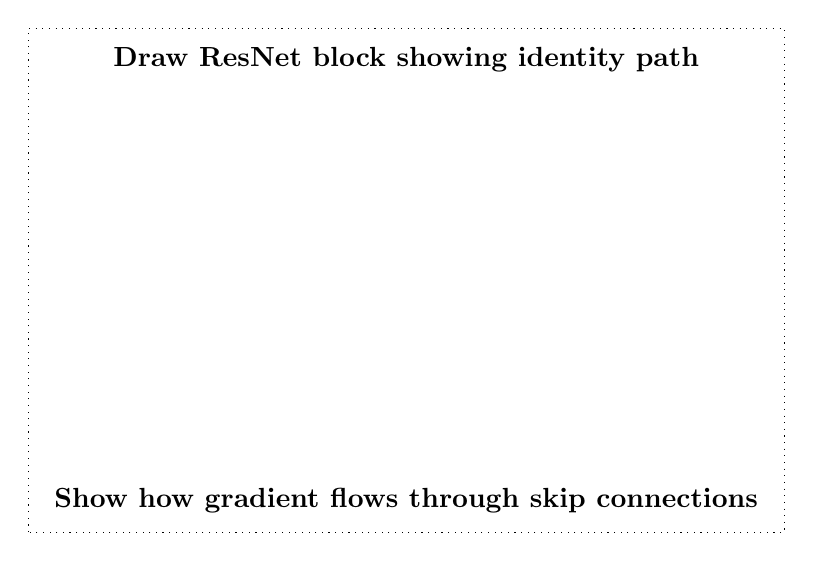
\begin{tikzpicture}[scale=0.8]
        % Space for ResNet block based on professor's explanation
        \draw[dotted] (0,0) rectangle (12,8);
        \node at (6,7.5) {\textbf{Draw ResNet block showing identity path}};
        \node at (6,0.5) {\textbf{Show how gradient flows through skip connections}};
    \end{tikzpicture}
    \end{center}
    
    \shortanswer
    
    \item The professor explained that ResNet "smooths the loss surface" and provides "robustness to slight changes in the weights." Explain this concept using the professor's reasoning about how identity transform provides robustness when weights change slightly. \hfill (7 marks)
    
    \mediumanswer
\end{enumerate}

\newpage
\paragraph{Question 2. ResNeXt and Multiple Pathways}{\hfill (20 marks)}\\
The professor described ResNeXt as extending ResNet "by utilizing multiple paths acting on the same input layer."

\begin{enumerate}[(a)]
    \item Compare ResNeXt with the inception module from GoogleNet as the professor discussed. Explain the key difference: "in inception module the filter sizes are different in different paths, whereas here in ResNeXt the sizes are the same." \hfill (8 marks)
    
    \mediumanswer
    
    \item The professor noted that ResNeXt "can provide better performance than ResNet however because of the multiple paths it is slower." Explain this trade-off and when you would choose ResNeXt over ResNet according to the professor's guidance. \hfill (7 marks)
    
    \mediumanswer
    
    \item Draw a ResNeXt block showing multiple functions $f_1(x), f_2(x), \ldots, f_{32}(x)$ acting on the same input as the professor illustrated, resulting in $x + f_1(x) + f_2(x) + \ldots + f_{32}(x)$. \hfill (5 marks)
    
    \shortanswer
\end{enumerate}

\newpage
\paragraph{Question 3. DenseNet Architecture}{\hfill (22 marks)}\\
Based on the professor's explanation: "We have residual connections not only skipping the next block but skipping to and making connections to all following blocks."

\begin{enumerate}[(a)]
    \item Explain DenseNet's approach to skip connections as described by the professor. Why does having "skip connections for all following layers" make it "a very dense network" and potentially "more difficult to implement"? \hfill (8 marks)
    
    \mediumanswer
    
    \item The professor mentioned that DenseNet "can provide better performance compared to ResNet" but wasn't sure "why it didn't become as popular as ResNet." Analyze the potential reasons for this based on implementation complexity and computational requirements. \hfill (8 marks)
    
    \mediumanswer
    
    \item Draw a DenseNet block showing how "from this layer we have skip connections to all following layers" as the professor described. Show at least 4 layers with their dense connections. \hfill (6 marks)
    
    \begin{center}
    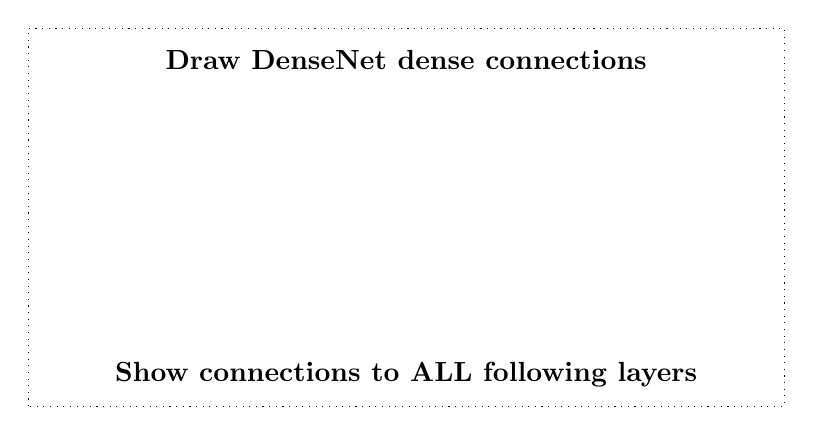
\begin{tikzpicture}[scale=0.8]
        % Space for DenseNet visualization
        \draw[dotted] (0,0) rectangle (12,6);
        \node at (6,5.5) {\textbf{Draw DenseNet dense connections}};
        \node at (6,0.5) {\textbf{Show connections to ALL following layers}};
    \end{tikzpicture}
    \end{center}
\end{enumerate}

\newpage
\paragraph{Question 4. Highway Networks and Gating}{\hfill (23 marks)}\\
The professor explained highway networks as providing "more flexibility to the network where we can modulate the skip connection."

\begin{enumerate}[(a)]
    \item Explain the highway network concept as described by the professor: "multiply the skip connection by a learnable function" and "multiply this by another function." Write the mathematical formulation the professor presented. \hfill (10 marks)
    
    \mediumanswer
    
    \item The professor showed how highway networks use gating: "t controls the information coming through here and with this we are also controlling how much x is propagated to the next layer." Explain this gating mechanism and how it differs from simple residual connections. \hfill (8 marks)
    
    \mediumanswer
    
    \item The professor noted that "highway networks were not as common as ResNets but the idea of gating is actually utilized in many different architectures." Give examples of where this gating concept is used and why it's important. \hfill (5 marks)
    
    \shortanswer
\end{enumerate}

\newpage
\paragraph{Question 5. Binary Networks and Efficiency}{\hfill (25 marks)}\\
Based on the professor's discussion: "In binary networks people are trying to replace real valued weights with binary weights and this would get rid of multiplication."

\begin{enumerate}[(a)]
    \item Explain the motivation for binary networks as the professor described: the need to "run these networks on low resource devices edge devices" where "it will be very difficult to run and execute deep architectures requiring a lot of memory." \hfill (8 marks)
    
    \mediumanswer
    
    \item The professor mentioned specific trade-offs: "we get 30 times around 30 times gain in terms of memory but we lose some accuracy." Calculate the memory savings for a network with 10 million 32-bit parameters when converted to binary, and explain when this trade-off is acceptable. \hfill (10 marks)
    
    \mediumanswer
    
    \item The professor explained that "if you change the input to binary and work only with binary values throughout the network then actually in addition to obtaining significant memory gain you can actually get very large gain in running time." Explain why binary operations are faster and when this approach is practical. \hfill (7 marks)
    
    \mediumanswer
\end{enumerate}

\newpage
\paragraph{Question 6. Introduction to Sequence Problems}{\hfill (35 marks)}\\
The professor introduced sequence modeling: "We have many problems where we have a sequence we need to process that sequence sequentially."

\begin{enumerate}[(a)]
    \item Classify the following problems according to the professor's framework (one-to-one, one-to-many, many-to-one, many-to-many) and explain your reasoning: \hfill (15 marks)
    \begin{itemize}
        \item Image captioning (which the professor said is "a very good example" of one-to-many)
        \item Spam detection (professor's example of many-to-one)
        \item Language translation (professor's example with "Turkish" to "English")
        \item Online speech recognition ("live speech recognition")
        \item Character recognition in a sequence
    \end{itemize}
    
    \journalspace
    
    \item The professor emphasized that in sequence problems "the information at a certain point might depend on the information we have seen so far." Explain why this context dependency makes traditional CNNs and MLPs insufficient for sequence modeling. \hfill (10 marks)
    
    \mediumanswer
    
    \item Compare feedforward networks with RNNs as the professor explained: "In feedforward network we don't have that option but the network has seen for the previous input we don't know." Draw both architectures showing how RNNs provide "memory capacity" through recurrent connections. \hfill (10 marks)
    
    \begin{center}
    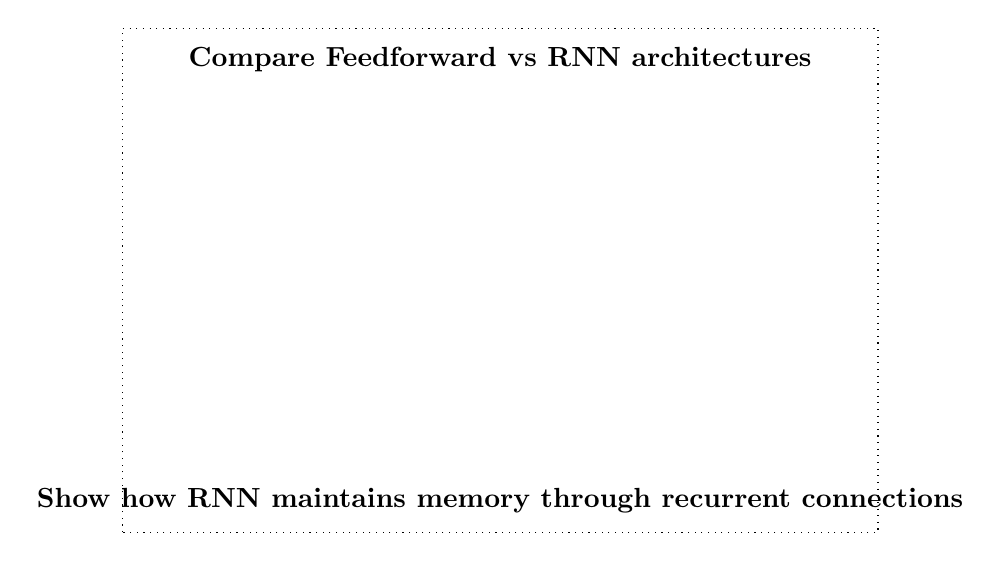
\begin{tikzpicture}[scale=0.8]
        % Space for comparison diagram
        \draw[dotted] (0,0) rectangle (12,8);
        \node at (6,7.5) {\textbf{Compare Feedforward vs RNN architectures}};
        \node at (6,0.5) {\textbf{Show how RNN maintains memory through recurrent connections}};
    \end{tikzpicture}
    \end{center}
\end{enumerate}

\vfill
\begin{center}{\bf END OF PAPER}\end{center}
\end{document}